\chapter{Analyser}
\label{chp:Analyser}
The flash analyser now outputs values at 125Hz, which is a mixture of various lights and noise. The next step is to create a real-time binary classification algorithm to convert the incoming samples into a logical value: Activity detected, or no activity detected. The detection algorithm should be designed with certain goals in mind:
\begin{itemize}
	\item \textbf{High true positive ratio} - The system does not fulfil it's purpose if it is unable to reliably detect bypassing objects.
	\item \textbf{Low false positive ratio} - The system is useless if it classifies everything as activity. This would result in the light being on all the time and therefore, no energy being saved.
	\item \textbf{Fast response time} - If the algorithm manges detect every bypassing person correctly, but it only triggers a detection when the user has already passed the light, then the system does not fulfil its purpose.
	\item \textbf{Low computational complexity} - If the algorithm uses too much calculations per incoming sample, the system would require a strong processor to analyse all incoming data. This makes the system expensive, if it where to eventually get implemented in the real world.
\end{itemize}
This chapter is separated in three parts. The first part shows what signals are received by the photo diode. The second part explains what methods considered to remove unwanted signals from the signal. The final part of this chapter what considerations where mode to determine threshold of the binary classifier.

\section{Received signals}
In an ideal world, the dark sensing system only perceives light it emits itself, reflected by the environment. The previous chapter already showed that this is not the case. Several other factors are influencing the measurements. Equation \ref{eq:Pd_light} has been devised and contains the most common signals the photo diode $PD$ might receive. Each term of the equation will be discussed briefly while pointing out what this signal looks like.

\begin{equation}
\label{eq:Pd_light}
PD = I_{L} \alpha + \sum_{i=1}^n I_{Edc_{n}} \beta_{n} + \sum_{i=1}^n I_{Eac{_n}} \gamma_{n} + N_{50Hz} + N(\mu,\sigma^2)
\end{equation}

$I_{L}$ represents the light emitted by the light. This gets multiplied with $\alpha$, which represents the environment from the point of view of the system. These two terms represents the ideal response. The expected frequency of $\alpha$ should lie between XHz and YHz for by passing pedestrians, as shown in chapter \ref{Model}. The goal of the complete algorithm is to isolate $\alpha$ and detect significant changes in it real-time.

The next term, $\sum_{i=1}^n I_{Edc_{n}}$, represents all constant, but slowly changing light sources in the area. An example of this is moonlight. Moonlight illuminates the surrounding area, but slowly changes over time because moon moves over time, or clouds blocking the moonlight. $\beta_{n}$ represents the environment from the point of view of the moon.
	
$\sum_{i=1}^n I_{Eac{_n}}$ represent all fluctuating light sources in the area. Most lights connected to the power grid fall into this category. They typically turn on and off at 100Hz in Europe. Some of the light produced by these source could reflect of off the environment $\gamma_{n}$ and reach the system and therefore influence the received signal.

Another term in the equation is $N_{50Hz}$, which represents 50Hz noise from the powergrid. As long as the system is connected to the grid, some 50Hz components will be seen in the system. Especially if amplified 1000 times.

the final term, $N(\mu,\sigma^2)$, represents the noise on the measurements not created by the "predictable" sources listed above. This noise originates from the imperfections of the platform and electromagnetic noise in the environment. In the previous chapter it was shown that the noise could be approximated with a Gaussian curve and its therefore represented by its mean ($\mu$) and variance ($\sigma^2$).

\section{Filter methods}
The goal of the filters is to get rid of unwanted signals in order to make the detection of $\alpha$ easier. Several digital filters types have been considered, each with different goals mind. The effectiveness (or failure) of each proposed filter will be shown, where possible, with the help of the signals shown in figure \ref{Original_signal}. (a) shows an optimistic case with an original SNR of 18.5. (b) shows a harder case with an original SNR of 10.5. This figure will display the filter working in a much harsher condition.

\begin{figure}
	\centering     %%% not \center
	\label{Original_signal}
	\subfigure[]{\label{fig:original_good}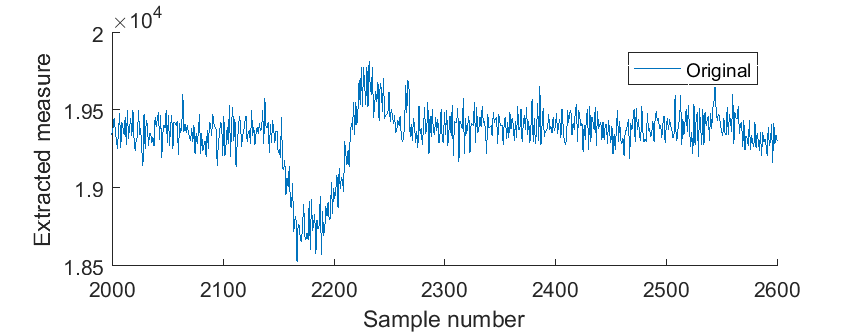
\includegraphics[width=60mm]{pics/Original_good.png}}
	\subfigure[]{\label{fig:Original_bad}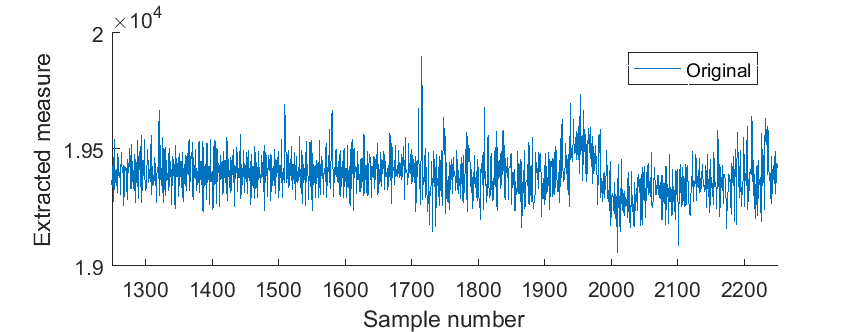
\includegraphics[width=60mm]{pics/Original_bad.png}}
	\caption{Two signals of a person walking underneath the set-up. Figure (a) shows an optimistic case with an SNR of 18.5 and (b) shows a harder scenario with an SNR of 10.5.}
\end{figure}

\subsection{Low-pass filters}
A lowpass filter can be used to remove $I_{Eac{_n}}$ and $N_{50Hz}$ from the measured signal as their frequencies are far removed from the signal we are interested in $\alpha$ (0.1 - 2Hz). Low-pass filters have one big downside for the system. They introduce a delay in the signal when used which is bad for the overall response time. Several filters have been tested. The final result is shown in figure \ref{lowpass_example} and is a second order IIR lowpass with its corner frequency at $XHz$. 

With this filter, the complete $N_{50Hz}$ component of the signal is removed and in most cases, $I_{Eac{_n}}$ is removed as well. We are however unable to grantee the removal of $I_{Eac{_n}}$ because of possible signal aliasing.

Signal aliasing is a phenomenon which occurs if the sample rate $F_{s}$ of a system is too compared to the signal being sampled. If $F_{s}$ is smaller then twice the frequency of then the sampled signal, the signal will appear as another frequency instead, an alias. This frequency is called $F_{alias}$ and can be calculated with equation \ref{Falias}, where $n$ is the closest integer mutiple of $F_{s}$ to the signal being aliased ($F_{Iac}$).

\begin{equation}
\label{Falias}
	F_alias = |F_{s} * n - F_{Iac}|
\end{equation}

Almost all lights have a flicker frequency higher than half the sample rate of the system and will therefore alias. In Europe most lights have blink frequencies which are multiples of $50Hz$ (frequency of the power grid) and will therefore show up with an alias frequency of $25Hz$. This frequency is can still be removed with the used low-pass filter. There is however no grantee that all lights will blink at a multiple of $50Hz$. In the Americas for example the grid is powered at $60Hz$. The chanse is very high that a light there typically flickers at $120Hz$, which will alias at $5Hz$. This frequency is too low for the low pass filter to remove and will have to be death with in another way (if it occurs).

\begin{figure}
	\centering     %%% not \center
	\label{lowpass_example}
	\subfigure[]{\label{fig:lowpass_good}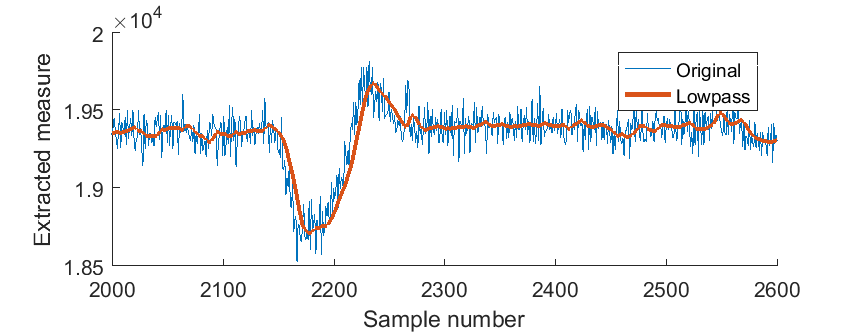
\includegraphics[width=60mm]{pics/lowpass_good.png}}
	\subfigure[]{\label{fig:lowpass_bad}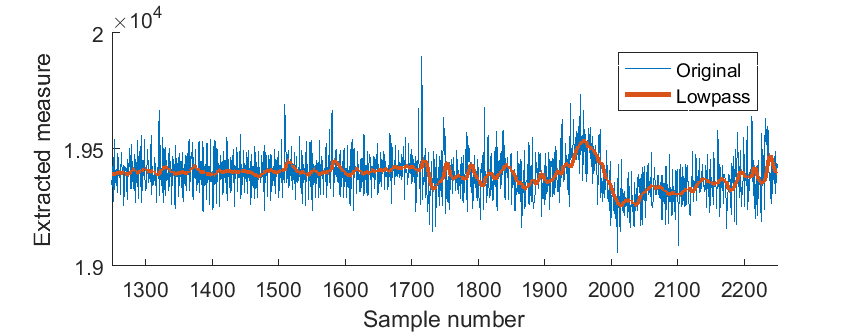
\includegraphics[width=60mm]{pics/lowpass_bad.png}}
	\caption{A lowpass filter ($F_{cutoff} = 5Hz$) applied to the two example signals. The SNR for signal (a) increased to 76.3 from 18.4 and the SNR of signal (b) increased to 12.6 from 10.5.}
\end{figure}

\subsection{Highpass filters}
Highpass filters can be used to remove $I_{Edc_{n}}$ from the signal. This is in this specific case very hard as the frequency we are interested in is very close to 0 compared to our sampling rate. It works, but it takes the filter a very long time to settle if a permanent change occurs in the environment. An example of this can be seen in figure X. In the figure a step is introduced at $t = 1000$, the signal has only settled after 11000 samples (90 seconds), which is not acceptable for the application. For this reason, the high pass filter is not part of the final algorithm.

\subsection{Moving average filters}
A moving average can be used to reduce $N(\mu,\sigma^2)$ and the remaining $F_{allias}$. A moving average is effectively a simple low pass filter with specific frequencies being removed completely at $\frac{F_s}{n}*x$, where $n$ is the number of tabs of the moving average and $x$ any integer greater than 0. Therefore a make shift filter can be created instantly if $F_{alias}$ is known, with $n = \left|\frac{F_{s}}{F{alias}}\right|$.

$F_{alias}$ could be determined with the help of a Fourier transformation and then filtered away with a make-shift moving average. Yes, the Fourier transform would cost a lot of computation power which is against our goal of creating a computationally light algorithm, but the transform wouldn't have to be ran every sample. It is probably good enough to run it once every 10 minutes, to check if $F_{alias}$ has been changed.

Another advantage the moving average brings is, that if the resulting noise is Gaussian, the noise gets reduced by a factor $\sqrt{(n)}$, where n is the number of tabs in the filter. It was therefore considered to scale the moving average, based on the current standard deviation of the noise with the help of equation \ref{eq:SNR_movavg}. The presented formula calculates $n$, so that the 

This method has two huge downsides. The first is that a moving average, capable of changing every incoming sample is computational expensive. If $n$ changes, then the full moving average needs to be re-evaluated ($n$ summations, 1 division)) instead of using a simple update rule (1 summation, 1 division). Another downside is that if $n$ gets too large, the response time of the system go down. For these two reasons, the scaling moving average was not implemented in the final algorithm.

\begin{equation}
\label{eq:SNR_movavg}
\frac{signal}{noise} = 1 = \frac{\mu * ss}{T * \frac{\sigma}{\sqrt{n}}} \Rightarrow n = \left(\frac{T * \sigma}{\mu*ss}\right)^2
\end{equation}

\begin{figure}
	\centering     %%% not \center
	\label{movavg_example}
	\subfigure[]{\label{fig:lowpass_good}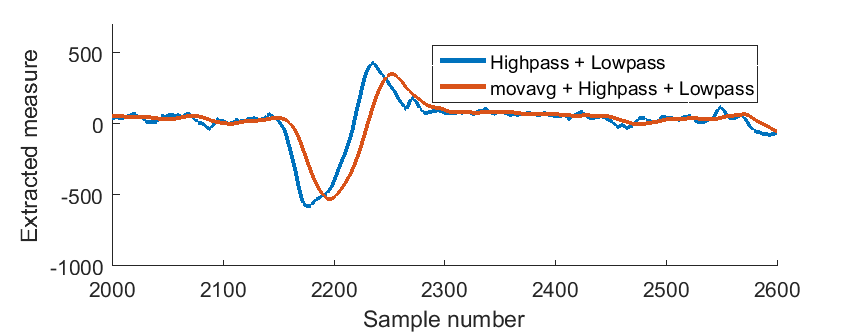
\includegraphics[width=60mm]{pics/movavg_good.png}}
	\subfigure[]{\label{fig:lowpass_bad}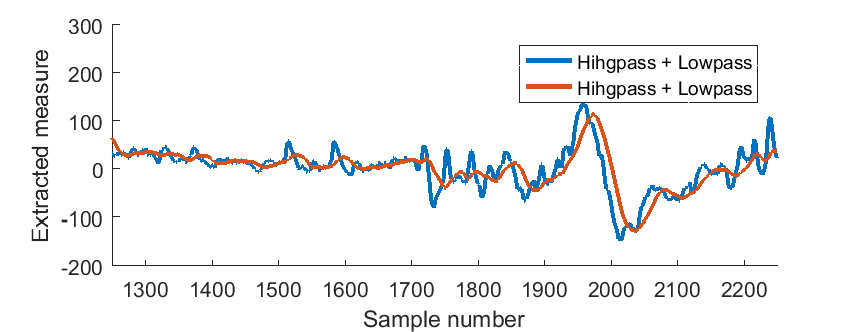
\includegraphics[width=60mm]{pics/movavg_bad.png}}
	\caption{A 10 tabs moving average applied to the two filtered example signals. The SNR for signal (a) increased to 80.1 from 76.3 and the SNR of signal (b) decreased slightly from 12.6 to 12.5.}
\end{figure}

\subsection{Differential filter}
The differential filter makes use of the fact that the system is not only able to sample when the light is turned on. Instead, It is possible to take samples while the light is turned off, to obtain $PD_{dark}$. This signal represents all the signals in the environment we are not interested in. If this signal is obtained very close to in time relative to $PD$ ($20\mu s$), then we can assume that all fluctuating sources in both, $PD$ and $PD_{dark}$, are equal. It's therefore possible to subtract the two signals, which would result in the filtered signal shown in equation \ref{eq:Pd_light_dark}.

\begin{equation}
\label{eq:Pd_dark}
PD_{dark} = \sum_{i=1}^n I_{Edc_{n}} \beta_{n} + \sum_{i=1}^n I_{Eac{_n}} \gamma_{n} + N_{50Hz} + N(\mu,\sigma^2)
\end{equation}

\begin{equation}
\label{eq:Pd_light_dark}
PD - PD_{dark} = I_{L} \alpha + N(0,\sigma^2 + \sigma^2_{dark})
\end{equation}
There are several downsides to this filtering method. The first is that we are subtracting two separate measures of the same noise signal. This leads to a higher variance on the complete signal and therefore a higher noise level. Another downside of this method is that it does not work properly with the current hardware set-up because the $PD_{dark}$, on its own, is below the sensitivity threshold of the receiver and is therefore unmeasurable, unless there is a lot of stray light in the area.

\subsection{Filter overview}
Several methods for removing unwanted parts of the received signal have been presented and summarised in table \ref{filtersOverview}. The final solution implements only the low pass filter and the moving average scaling based on $F_{alias}$. Figure X shows the remaining distribution of noise after the two implemented filters for both, the hard case and the easy case.

\begin{table}[]
	\hskip-2.0cm
	\label{filtersOverview}
\begin{tabular}{l|lll}
	Filter type                                                        & Goal                                                                                     & Notes                                                                                                                             & In final algorithm? \\ \hline
	Low pass filter                                                    & \begin{tabular}[c]{@{}l@{}}Filter $I_{Eac}$ and \\ $N_{50Hz}$\end{tabular}               & \begin{tabular}[c]{@{}l@{}}Can't guarantee the removal of $I_{Eac}$\\ due to signal aliassing\end{tabular}                        & Yes                 \\ \hline
	High pass filter                                                   & Filter I\_\{Edc\}                                                                        & \begin{tabular}[c]{@{}l@{}}Slow step response and therefore\\ unusable\end{tabular}                                               & No                  \\ \hline
	\begin{tabular}[c]{@{}l@{}}FFT based\\ moving average\end{tabular} & \begin{tabular}[c]{@{}l@{}}Filter $F_{alias}$ and \\ reduce $N(\mu,\sigma)$\end{tabular} & \begin{tabular}[c]{@{}l@{}}Works, as long as $F_{alias}$ is not too\\ close to $I_{L} \alpha$\end{tabular}                        & Yes                 \\ \hline
	\begin{tabular}[c]{@{}l@{}}SNR based\\ moving average\end{tabular} & reduce $N(\mu,\sigma)$                                                                   & \begin{tabular}[c]{@{}l@{}}Worked, but introduced huge delays for high\\ $\sigma$ and was is computational intensive\end{tabular} & No                  \\ \hline
	$PD-PD_{dark}$                                                     & \begin{tabular}[c]{@{}l@{}}Filter $I_{Eac}$, $N_{50Hz}$\\ and $I_{Edc}$\end{tabular}     & \begin{tabular}[c]{@{}l@{}}Only worked in illuminated enviroments\\ which made it unriliable to filter $N_{50Hz}$\end{tabular}    & No                 
\end{tabular}
	\caption{Overview of the filter methods described in this section}
\end{table}

\section{Detection threshold}

There are several reasons why the threshold can't be static and has to self adjust overtime:
\begin{itemize}
	\item $I_dc$ - 
	\item 
\end{itemize}


\subsection{Naive thresholds methods}


\subsection{Standard deviation based threshold}
A threshold can be made based on the standard deviation of the signal. This method in literature is called the blabla method \cite{@}.

A delay can be added between the threshold and X, to increase detection ratio and detecting speed.

If the delay is too long it might increase the false positive ratio if the signal is slowly drifting upwards or downwards.

\subsection{Variance based threshold}
A threshold can be made based on the variance. By comparing 




%\begin{figure}
%	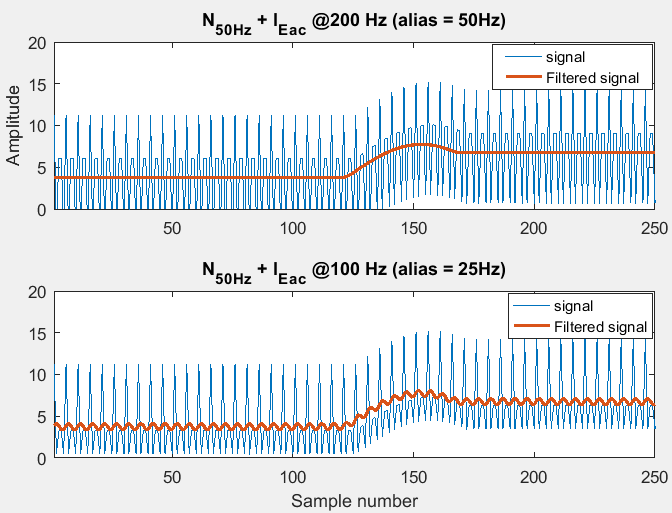
\includegraphics[width=\textwidth]{pics/FirFilter_vs_allias.png}
%	\caption{A low-pass filter, filtering the $I_{Eac}$ and $N_{50Hz}$ signals.}
%	\label{fig:FilterVSAllias}
%\end{figure}


\subsection{Detection threshold}
A naive solution to this problem would be to sample a set amount of values when there are no objects in sight. Then, take the maximum and minimum of the sampled values and if the signal ever moves out of the range of the found values, activity is detected. Even though this might work consistently in a dark room (lab environment with no lights), it fails to work in a more realistic environment. If we for example introduce a slowly rising $I_{Edc}$ (e.g. moonlight), then the signal will eventually peak above the current maximum value and trigger a false detection.

Another way of tackling this problem would be to allow the minimum and maximum thresholds to move up and down with the mean of the signal. This results in two thresholds moving up and down together with the mean of the signal, and therefore ignores the slow changing $I_{Edc}$. The downside of this solution is that if the noise level ($N(\mu,\sigma^2)$) where to increases, then the signal would still cross the set threshold and trigger a false detection. The opposite is also true. If the noise level decreases, then the threshold would not scale back automatically and thus making it "deaf" to smaller changes in the signal.

This problem can be solved using the standard deviation of the signal as thresholds instead. A standard deviation scales up and down based on the deviation from the mean, meaning that if a lot of noise is present in the signal, then the detection borders would scale up and vice versa. The detection borders could be set on $\mu\pm T\sigma$, where $\mu$ is the mean, $\sigma$ is the standard deviation and $T$ is a factor determining width of the threshold

Using this method has another benefit. As the noise in our system ($N(\mu,\sigma^2)$) can be approximated with a normal curve (see section \ref{subsec:noise}), it allows us to control the amount of false positives perceived by the system by adjusting the $T$ parameter. How $T$ influences the chance of a false positive can be seen in table \ref{tab:Tresholds}.

\begin{table}
	\centering
	\label{tab:Tresholds}
	\begin{tabular}{cccl}
		\hline
		T   & Chance false positive & Single occurrence @125 Hz & Double occurrence @125Hz\\ \hline
		2   & 4.550026\%            & 0.18s                     & 0.69 days               \\
		3   & 0.269979\%            & 2.96s                     & 198.5 days              \\
		4   & 0.006334\%            & 126.3s                    & 1001 years              \\
		5   & 0.000057\%            & 1178.2s                   & 12199827 years          \\ \hline
	\end{tabular}
	\caption{Chance of a false positive occurring for several values of T, how often this would happen}
\end{table}



%Discuss fixed threshold
%note that this does not adjust to a slowly changing I_DC
%discuss variable threshold with mu and sigma
%show that this kind of works.
%show how scaling m influcences algorithem

\begin{figure}
	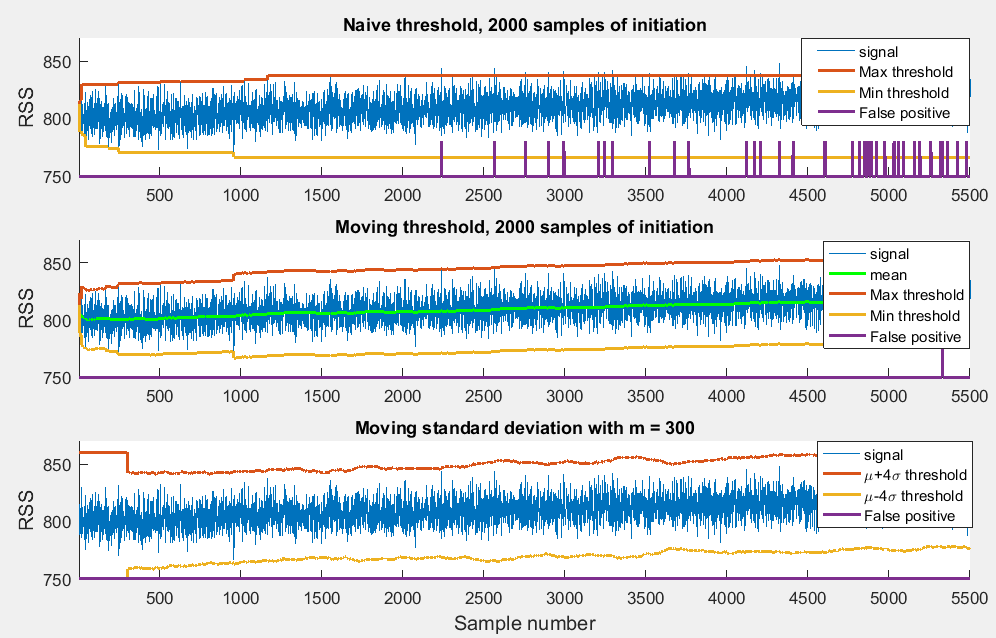
\includegraphics[width=\textwidth]{pics/NaiveVSsigmaThreshold.png}
	\caption{An example of how the discussed threshold algorithms respond to a slowly rising noisy signal.}
	\label{fig:Threshold}
\end{figure}

\begin{figure}
	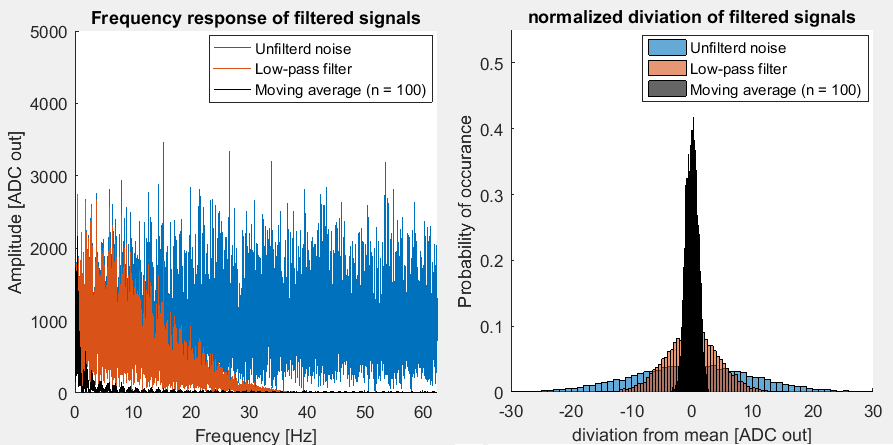
\includegraphics[width=\textwidth]{pics/FiltersVsNoise.png}
	\caption{Frequency response of the noise, the noise when filtered with a low-pass filter, and then noise when filtered with a moving average.}
	\label{fig:FilterVsNoise}
\end{figure}

\subsection{Algorithm overview}


\begin{figure}
	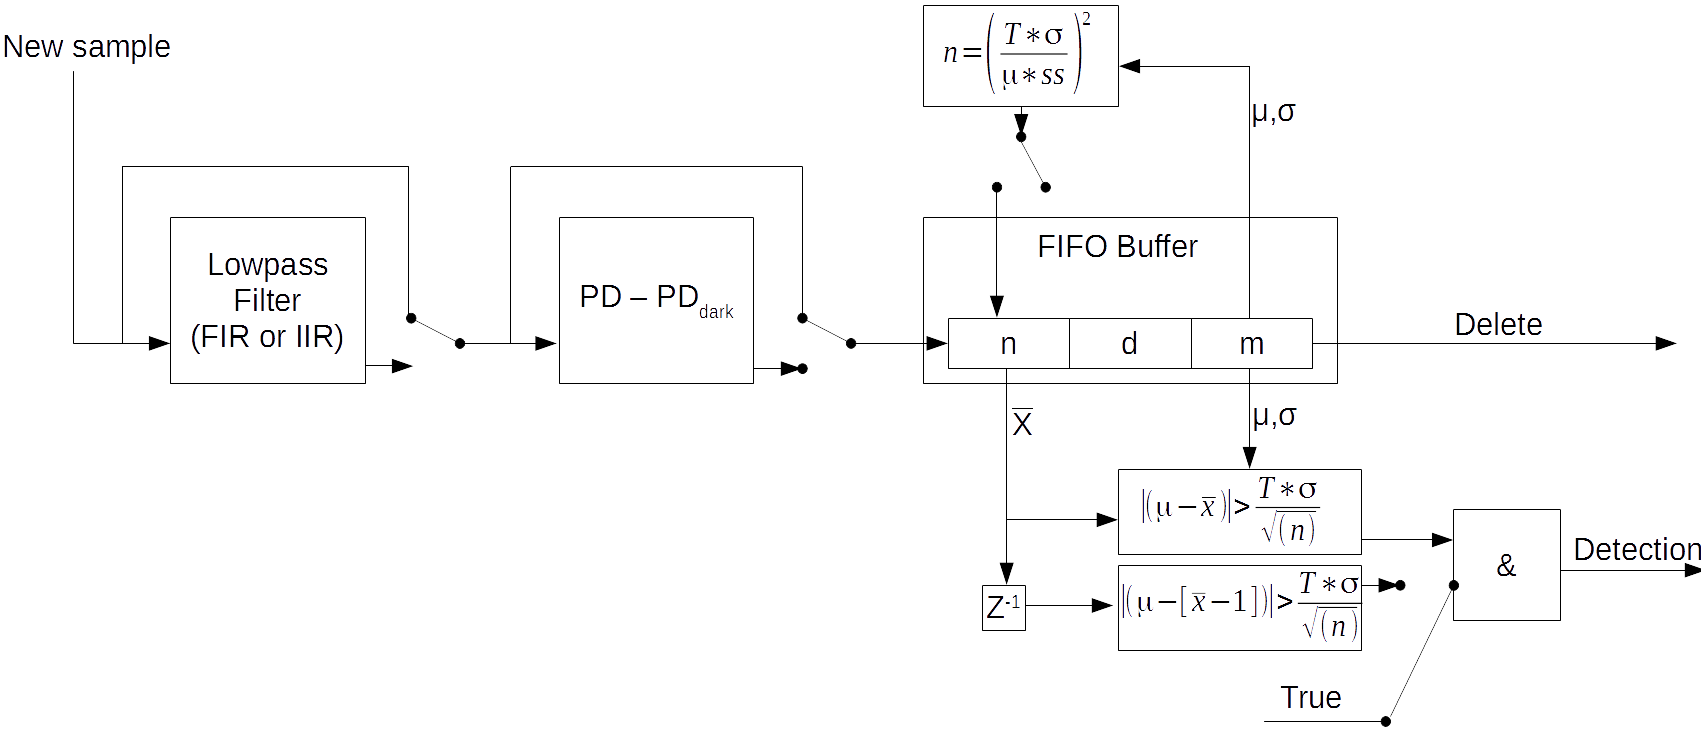
\includegraphics[angle=90,width=\textwidth]{pics/allSTDbasedAlgorithms_expanded.png}
	\caption{Overview of the algorithm.}
	\label{fig:fullAlgorithm}
\end{figure}
